% =====================================================================
%  IEEE Sensors Letters — v2 초안 (2026-08-09)
%  v1(paper/IEEE_Sensors_letters_overleaf.tex, 2026-07-21) 에서 형식만 재사용.
%  본문 문장은 전부 새로 썼다.
%
%  숫자 출처: results/v2/train_encoder_final.json, train_image_cnn_{head,max}_final.json,
%             cmp_*_FINAL.json, posthoc_subgroups_final.json, posthoc_vs_imgcnn_head.json,
%             export_onnx.json, pi_{ear,ours,image_cnn_max,image_cnn_head}_480p.json,
%             cmp_vpres_vs_vdrop.json
%
%  🔴 투고 전 검색해서 0건인지 확인: privacy-preserving / identity / irreversible /
%     anonymized / causal / "first" / "only" / 420x / 99%
% =====================================================================

\documentclass{IEEE_lsens}
% ⚠️ IEEE_lsens.cls 는 저장소에 없다. Overleaf 에서만 조판된다.

\usepackage{textcomp}
\usepackage[noadjust]{cite}
\usepackage[T1]{fontenc}
\usepackage{amsmath}
\interdisplaylinepenalty=2500
\usepackage[cmintegrals]{newtxmath}
\usepackage{bm}
\usepackage{array}
\usepackage{url}
\usepackage{graphicx}
\graphicspath{{./}{paper_assets/}}
\usepackage{tikz}
\usetikzlibrary{arrows.meta, positioning, calc}

\providecommand{\hypersetup}[1]{\relax}
\providecommand{\texorpdfstring}[2]{#1}

\hyphenation{op-tical net-works semi-conduc-tor}

\begin{document}

\markboth{IEEE Sensors Letters}{0000000}

\IEEELSENSarticlesubject{Sensor Applications}

\title{Eye Blink Detection on Low-Dimensional Embeddings\\
for Real-Time Operation on Edge Hardware}

\author{\IEEEauthorblockN{Anonymous Author(s)}%
\IEEEauthorblockA{Affiliation withheld for double-blind review}%
\thanks{Corresponding author: withheld for review.}%
\thanks{Associate Editor: [TBD].}%
\thanks{Digital Object Identifier 10.1109/LSENS.XXXX.XXXXXXX}}
\IEEELSENSmanuscriptreceived{Manuscript received [Month] [Day], [Year];
accepted [Month] [Day], [Year]. Date of publication [Month] [Day], [Year];
date of current version [Month] [Day], [Year].}

\IEEEtitleabstractindextext{%
\begin{abstract}
Camera-based eye blink monitoring is increasingly deployed on
edge-class hardware, where the cost of the visual pipeline matters as
much as its accuracy. We detect blink events on a low-dimensional
representation: each frame is encoded once into a 16-dimensional
embedding, and the classification stage operates on a buffer of these
embeddings rather than on raw eye images. On a 57-subject subset of the
mEBAL2 database (27{,}758 events, subject-disjoint five-fold
cross-validation with three seeds), the proposed model reaches a PR-AUC
of $0.9886 \pm 0.0038$ against $0.9906 \pm 0.0037$ for an image-based
convolutional baseline equipped with the same temporal head. The paired
subject-clustered difference is $-0.0040$ (95\% CI $[-0.0063,-0.0020]$),
within a non-inferiority margin of $\delta = 0.02$ fixed before the
comparison, while using $5.7\times$ fewer parameters and $2.6\times$
fewer multiply--accumulate operations. On a Raspberry Pi~5 at
$640\times480$, the representation stage costs $0.86$~ms per frame
versus $2.04$~ms for the image-based baseline, but the end-to-end gain
is only 11\%: face and landmark detection accounts for 68--87\% of the
pipeline, and is therefore the binding constraint at the edge.
\end{abstract}
\begin{IEEEkeywords}
Eye blink detection, learned representation, embedding, temporal
convolutional network, edge computing, on-device inference.
\end{IEEEkeywords}}

\maketitle

% =====================================================================
\section{Introduction}

Spontaneous eye blinking is a low-cost behavioural signal with several
sensing applications. Blink rate and blink completeness are used as
indicators of ocular surface stress during prolonged screen work
\cite{rosenfield2011}, and blink dynamics feed drowsiness and attention
estimation. Because webcams are now permanently present in office and
in-vehicle settings, the practical question is less whether blinks can
be detected than at what cost they can be detected continuously, on the
device that already holds the camera.

Two families dominate. Landmark-based methods reduce each frame to a
geometric ratio such as the eye aspect ratio (EAR) \cite{soukupova2016};
they are essentially free once landmarks exist, but compress the eye
region to a single scalar and discard everything else. Image-based
convolutional methods classify the eye crop directly
\cite{daza2020,daza2024} and are more accurate, but pay a convolutional
cost over the full crop at every frame of the decision path. It is worth
noting that the original EAR formulation is not a fixed threshold: it
classifies a short temporal window of EAR values with a learned
classifier \cite{soukupova2016}. A comparison that defeats only a
thresholding rule therefore weakens its own baseline, and we report both
variants.

We take an intermediate position. Each frame is encoded once by a small
convolutional encoder into an embedding $z \in \mathbb{R}^{16}$, the
last 19 embeddings are held in a ring buffer, and a temporal
convolutional head classifies the window. The classification stage
operates on embeddings rather than raw eye images, and re-encoding is
never required: the per-frame encoding is reused by every window that
contains it.

Our contributions are threefold. (i) Under a single protocol --- the
same crops, the same temporal and classification head, the same folds,
seeds, threshold grid and bootstrap --- we compare two EAR variants, two
variants of a literature image-based CNN, and the proposed model, and
show that the proposed model is non-inferior to the strongest
image-based control at a margin fixed in advance, with $5.7\times$ fewer
parameters. (ii) We report a vertical-resolution ablation with a
confound-free control, which does not support the resolution argument
that motivated our encoder and instead indicates that a cheaper encoder
would suffice. (iii) We decompose per-stage latency of four methods on a
Raspberry Pi~5 under one harness, and quantify why a $2.4\times$
representation-stage advantage shrinks to 11\% end-to-end.

% =====================================================================
\section{Related Work}

Blink detection has been addressed with landmark ratios and learned
temporal windows \cite{soukupova2016}, per-frame convolutional
classifiers with score aggregation \cite{daza2020}, and sequence models
including convolutional recurrent and transformer architectures
\cite{daza2024,fodor2023}. Recent work moves to unconstrained
multi-person untrimmed video with a one-stage spatio-temporal
transformer, reporting 112~FPS for network forwarding on an NVIDIA~3090
GPU \cite{zeng2023}. That setting is complementary to ours: multiple
faces, long untrimmed video and GPU inference, against a single user,
event classification and edge-class hardware. We do not compare speeds
across these settings, since the detectors, frameworks and resolutions
differ.

% ⚠️ [검색요약] 상태의 인용 2건(arcaya2021, fodor2023) 이 이 문단에 있다.
%    **투고 전 원문 확인 필수.** arcaya2021 이 지연·파라미터를 실제로 보고하면
%    아래 문장을 그에 맞게 다시 써야 한다.
Embedded blink detection has been demonstrated on wearable hardware,
where a convolutional classifier improved over a thresholding rule while
keeping memory and battery overhead acceptable \cite{arcaya2021}. Beyond
such cases, however, the reported literature is difficult to place
alongside ours: most on-device studies evaluate drowsiness state rather
than blink events, so the label unit and the metric differ; those that
do report blink events typically give accuracy without latency,
operation counts or sustained throughput; and non-camera modalities such
as capacitive sensing change the input entirely
\cite{capacitive2024}. Within the scope of our search we did not find a
study reporting both event-level detection quality and a per-stage edge
latency breakdown for the same system, which is what we provide here.

Performing classification on a learned representation rather than on
pixels has been explored for blinks with a 3D autoencoder whose latent
code feeds a classifier \cite{nousias2025}. That work targets offline
analysis: the reported processing time for a 60~s recording is
135--225~s across their variants, i.e.\ none of them runs in real time,
although the hardware for that measurement is not stated in a form we
could verify. Our aim is the opposite end of the trade-off --- a
representation small enough that the encoder is no longer the dominant
cost on a general-purpose edge CPU.

% =====================================================================
\section{Proposed Method}

% ---------------------------------------------------------------------
% Fig. 1 — docs/v2/figures/fig1_architecture.svg 를 TikZ 로 재작성.
% 자립형. pdflatex 컴파일 검증 완료 (자연 크기 254.6 x 125.5 pt).
% 숫자 출처: results/v2/export_onnx.json
% ---------------------------------------------------------------------
\begin{figure}[!t]
\centering
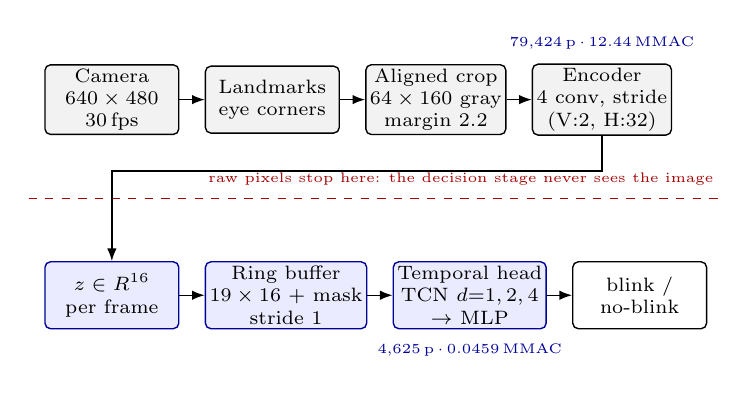
\begin{tikzpicture}[
  font=\scriptsize,
  box/.style  = {draw, rounded corners=2pt, minimum height=8.5mm,
                 minimum width=17mm, align=center, inner sep=1.5pt, line width=0.5pt},
  pix/.style  = {box, fill=black!5},
  vec/.style  = {box, fill=blue!8, draw=blue!60!black},
  ar/.style   = {-{Latex[length=1.6mm]}, line width=0.5pt},
  cost/.style = {font=\tiny, text=blue!60!black},
  node distance = 3.2mm
]
\node[pix] (cam)  {Camera\\$640\times480$\\30\,fps};
\node[pix, right=of cam]  (mesh) {Landmarks\\eye corners};
\node[pix, right=of mesh] (crop) {Aligned crop\\$64\times160$ gray\\margin $2.2$};
\node[pix, right=of crop] (enc)  {Encoder\\4 conv, stride\\(V:2, H:32)};
\node[cost, above=0.6mm of enc] {79{,}424\,p\,$\cdot$\,12.44\,MMAC};
\draw[ar] (cam) -- (mesh);   \draw[ar] (mesh) -- (crop);   \draw[ar] (crop) -- (enc);
\node[vec, below=16mm of cam] (z)   {$z\in\mathbb{R}^{16}$\\per frame};
\node[vec, right=of z]        (ring){Ring buffer\\$19\times16$ + mask\\stride 1};
\node[vec, right=of ring]     (head){Temporal head\\TCN $d{=}1,2,4$\\$\rightarrow$ MLP};
\node[cost, below=0.6mm of head] {4{,}625\,p\,$\cdot$\,0.0459\,MMAC};
\node[box, right=of head] (out) {blink /\\no-blink};
\draw[ar] (z) -- (ring);   \draw[ar] (ring) -- (head);   \draw[ar] (head) -- (out);
\path (enc.south) -- (head.north) coordinate[pos=0.5] (mid);
\draw[red!65!black, dashed, line width=0.6pt]
      ($(cam.west |- mid)+(-2mm,0)$) -- ($(out.east |- mid)+(2mm,0)$);
\node[font=\tiny, text=red!65!black, anchor=south east]
      at ($(out.east |- mid)+(2mm,0.4mm)$)
      {raw pixels stop here: the decision stage never sees the image};
\draw[ar] (enc.south) -- ++(0,-4.5mm) -| (z.north);
\end{tikzpicture}
\caption{Proposed pipeline. Each frame is encoded once into a
16-dimensional embedding; the 19-frame window is assembled from buffered
vectors rather than re-encoded, so the temporal head costs 0.37\% of the
per-frame compute. The head uses symmetric dilated convolutions and is
therefore not causal within the window, but it reads only frames already
in the buffer and adds no buffering latency. No decoder is deployed.}
\label{fig_pipeline}
\end{figure}

\subsection{Overview}
Fig.~\ref{fig_pipeline} shows the pipeline. A face landmark model
locates the eye corners in each frame; a rotation-aligned crop of both
eyes is resized to a fixed $64\times160$ grayscale image; an encoder
maps the crop to $z \in \mathbb{R}^{16}$; the last 19 embeddings and
their validity mask are held in a ring buffer; and a temporal
convolutional head followed by a small MLP emits a blink score. The
landmark coordinates are used only to derive the crop geometry and are
then discarded.

\subsection{Eye Crop Normalization}
The crop is centred on the midpoint of the two eye centres and rotated
so that the inter-ocular line is horizontal. Its width is set to
$2.2\times$ the inter-ocular distance and then resized to a fixed
resolution, so that the crop scale is normalized against changes in
camera distance. Pixel values are standardized per frame as
$(x-\mu)/\sigma$; this removes a global photometric shortcut that a
model could otherwise exploit instead of eyelid motion.

\subsection{Encoder Design and Vertical-Resolution Ablation}
The eyelid aperture is small relative to the crop: measured on our data,
the eyelid gap is $0.1201$ of the inter-ocular distance, i.e.\ about
$8.7$~px of the 64-px crop height. This observation motivated an
asymmetric encoder that reduces the horizontal axis by $32\times$ while
limiting the vertical total stride to $2$, on the reasoning that the
horizontal extent exists to hold two eyes side by side rather than to
carry resolution.

That reasoning is not supported by the data, and we report the test
rather than the argument. We built a confound-free control, denoted
\emph{vdrop}, identical in kernels, channels and horizontal stride but
with vertical total stride $16$, which reduces the eyelid gap at the
bottleneck to $0.55$~px and the convolutional cost from $12.41$ to
$3.44$~MMAC. The predicted collapse did not occur: the difference is
$+0.0010$ with a 95\% CI of $[-0.0032,+0.0069]$, and a sweep over
$D \in \{8,16,32,64\}$ was likewise indistinguishable. We keep the
higher-resolution variant because all downstream artefacts are built on
it and, as Section~\ref{sec_edge} shows, its extra cost is invisible
end-to-end --- not because it performs better.

\subsection{Temporal Modeling on Embeddings}
Re-encoding all 19 frames at every decision would multiply the encoder
cost by 19 and exceed the edge budget. Instead each frame is encoded
once and the window is assembled from buffered vectors. Because the
buffer carries 16 numbers per frame rather than a $64\times160$ crop,
the temporal head is small: three dilated convolutions ($d=1,2,4$)
followed by an MLP cost $0.0459$~MMAC per frame at stride~1, which is
$0.37\%$ of the per-frame total. Without the bottleneck --- for
instance with a 512-dimensional feature map --- the same head would cost
$2.36$~MMAC per frame, $51\times$ more. Frames in which the face is not
resolved have no crop; filling them with zeros would make ``no change''
indistinguishable from ``unknown'', so a validity mask is carried
alongside the buffer and masked positions are excluded from pooling.
The head is evaluated at stride~1: deciding only at window boundaries
would delay detection by up to 18 frames, i.e.\ $600$~ms at 30~fps.

\subsection{Deployment}
The encoder and both heads are compiled to ONNX, together $335$~KB. No
decoder is deployed.

% =====================================================================
\section{Experimental Setup}

\subsection{Dataset}
We use the RGB webcam stream of a 58-subject subset of the mEBAL2
database \cite{daza2024}, whose full release contains 180 subjects and
additional near-infrared channels that we do not use. The subset
combines 38 subjects from the 2020 acquisition and 20 subjects added in
2022. One subject (U18) is excluded because that session was recorded
with several people in frame and, whenever the primary subject was not
resolved, a neighbouring person was cropped instead --- affecting 31\%
of that subject's events. The remaining 57 subjects yield 27{,}758
events (13{,}820 blink, 13{,}938 no-blink) and 532{,}109 crops. An event
is a fixed 19-frame window.

\subsection{Protocol}
We use subject-disjoint five-fold cross-validation, stratified jointly
by event count and acquisition batch, with three seeds (15 runs).
Thresholds are selected on validation folds and results are reported on
held-out test folds. All methods share one implementation of the folds,
seeds, threshold grid and bootstrap. As an independent check that the
runs are otherwise identical, the configurations differ only in the
frontend and output paths, and the two EAR baselines --- which do not
depend on the frontend --- are bit-identical across the three runs.

\subsection{Baselines}
Five methods are compared. \emph{EAR-rule} thresholds the relative EAR
drop within the window. \emph{EAR-head} lifts the EAR features and feeds
the same temporal and classification head used by our model.
\emph{Image-CNN (max)} is the convolutional detector proposed by the
database authors \cite{daza2020}, with sequence scoring by the maximum
of per-frame scores as in the original. \emph{Image-CNN (+head)}
replaces that aggregation with our temporal head, leaving only the
frontend different. \emph{Ours} encodes the crop to an embedding and
uses the same head.

Two choices are deliberate. EAR is computed from the landmarks
distributed with the database, so all methods share one detector and one
face-selection rule; and we use the stronger of two EAR variants, the
relative-drop formulation, which is $0.17$~AUC above a minimum-EAR
rule. The image-based backbone is not our design: it is the architecture
the database authors proposed and benchmarked \cite{daza2020}, which
blocks the objection that we selected a weak baseline. That backbone was
originally trained with per-frame open/closed labels, whereas our
protocol provides one label per 19-frame window; the max-pooling variant
is thus trained under multiple-instance supervision and its performance
here may underestimate the original method.

\subsection{Metrics}
The primary metric is PR-AUC, with ROC-AUC, accuracy, precision, recall
and $F_1$ reported alongside. Comparisons use the paired
subject-clustered bootstrap of the difference, with a non-inferiority
margin $\delta = 0.02$ fixed before the comparisons were run. Cost is
reported as parameters, model size, multiply--accumulate operations per
frame, per-stage latency, end-to-end latency percentiles, sustained
frame rate, peak resident memory and CPU utilization.

\subsection{Edge Platform}
Measurements are taken on a Raspberry Pi~5 (16~GB, active cooling)
running Debian~13 and Python~3.11, with ONNX Runtime restricted to two
intra-op threads and spinning disabled, and the landmark model without
attention refinement. The CPU governor is set to \texttt{performance}
and each mode is measured over 300~s of sustained $640\times480$
playback at 30~fps.

% =====================================================================
\section{Results and Discussion}

% ---------------------------------------------------------------------
% Table I — 확정값. 출처: results/v2/train_encoder_final.json,
% train_image_cnn_{head,max}_final.json, export_onnx.json
% EAR-head 5,009 params / 0.0462 MMAC 는 export_onnx.json ear_head 블록 (2026-08-09).
% ---------------------------------------------------------------------
\begin{table*}[!t]
\caption{Blink Detection Performance and Static Cost.
Subject-Disjoint 5-Fold $\times$ 3 Seeds, 57 Subjects, 27{,}758 Events.
Mean $\pm$ Standard Deviation over Folds.}
\label{table_main}
\centering
\renewcommand{\arraystretch}{1.25}
\begin{tabular*}{\textwidth}{l@{\extracolsep{\fill}}cccccccc}
\hline\hline
Method & PR-AUC & ROC-AUC & Acc & Prec & Rec & F1 & MMAC & Params\\
\hline
EAR (rule)              & 0.8931 $\pm$ 0.0136 & 0.9169 $\pm$ 0.0146 & 0.8505 & 0.8268 & 0.8878 & 0.8550 & $\sim$0 & 0\\
EAR + temporal head     & 0.9724 $\pm$ 0.0096 & 0.9738 $\pm$ 0.0113 & 0.9276 & 0.9312 & 0.9228 & 0.9268 & 0.0462 & 5{,}009\\
Image-CNN (max) \cite{daza2020} & 0.9114 $\pm$ 0.0291 & 0.9404 $\pm$ 0.0207 & 0.8917 & 0.8526 & 0.9480 & 0.8971 & 31.81 & 470{,}561\\
Image-CNN (+ our temporal head) & \textbf{0.9906 $\pm$ 0.0037} & \textbf{0.9930 $\pm$ 0.0036} & 0.9651 & 0.9713 & 0.9584 & 0.9644 & 31.85 & 476{,}161\\
\textbf{Ours} ($D=16$)  & 0.9886 $\pm$ 0.0038 & 0.9914 $\pm$ 0.0037 & 0.9620 & 0.9605 & 0.9636 & 0.9618 & \textbf{12.49} & \textbf{84{,}049}\\
\hline\hline
\end{tabular*}
\vspace{0.5mm}
{\footnotesize
The MMAC column counts operations \emph{after} landmarks are available.
All five methods share the same landmark frontend, whose cost is
reported separately in Table~\ref{table_edge}; ``$\sim$0'' for the EAR
rule means a few divisions on six landmark points, not a free method.
Image-CNN (max) aggregates per-frame scores by their maximum, following
\cite{daza2020}; that model was trained there with per-frame
open/closed labels, whereas our protocol supplies one label per
19-frame window, so its performance here may be an underestimate of the
original method. Bold marks the best value in each column.}
\end{table*}

\subsection{Detection Accuracy}
Table~\ref{table_main} reports the confirmed runs. The best PR-AUC in
the table is not ours: the image-based backbone with our temporal head
reaches $0.9906 \pm 0.0037$ against our $0.9886 \pm 0.0038$. Our claim
is about cost, not accuracy. The paired subject-clustered difference
between the two is $-0.0040$ with a 95\% CI of $[-0.0063,-0.0020]$,
which clears the pre-registered margin $\delta = 0.02$ by a wide
factor; on the same folds the proposed model uses $5.7\times$ fewer
parameters ($84{,}049$ against $476{,}161$) and $2.6\times$ fewer
multiply--accumulate operations per frame.

We report two estimators of that difference, because they answer
different questions. The subject-clustered bootstrap asks what would
happen with a different sample of 57 subjects and excludes zero. The
run-mean over folds and seeds asks what would happen on retraining, and
gives $-0.0019 \pm 0.0024$ against a within-fold seed standard deviation
of $0.0031$. In other words, the gap is stable under subject
resampling, yet of the same magnitude as ordinary training variation,
and on either estimator it is far inside $\delta$.

The comparison against the literature aggregation must be read
carefully. Our model is $+0.0766$ above Image-CNN (max), CI
$[+0.0556,+0.0986]$ --- but attaching our temporal head to that same
backbone yields $+0.0806$, CI $[+0.0592,+0.1028]$. The gap is therefore
attributable to temporal modelling, not to the representation, and the
first number should never be quoted alone. The same pattern separates
the two EAR variants. Against the stronger EAR baseline our model is
$+0.0151$, CI $[+0.0106,+0.0203]$; all 15 runs were compared against
that stronger variant.

% ---------------------------------------------------------------------
% Fig. 2 — src/v2/make_fig2_subgroups.py 로 생성, 값은
% results/v2/posthoc_subgroups_final.json 에서 읽는다.
% ⚠️ 3.4 in 배치에서 2줄 y축 라벨이 잘리는지 Overleaf 에서 확인할 것.
% ---------------------------------------------------------------------
\begin{figure}[!t]
\centering

\includegraphics[width=\columnwidth]{fig2_subgroups.pdf}
\caption{Paired subject-clustered bootstrap difference in PR-AUC
(ours $-$ EAR + temporal head) by acquisition batch and eyewear, with
95\% confidence intervals; event-weighted pooling, 2{,}000 resamples.
The dashed line marks the pre-registered non-inferiority margin.}
\label{fig_subgroups}
\end{figure}

\subsection{Robustness across Conditions}
Fig.~\ref{fig_subgroups} shows the comparison against the stronger EAR
baseline within subgroups. The advantage holds in all five: $+0.0151$
overall, $+0.0118$ and $+0.0256$ for the 2020 and 2022 acquisition
batches, and $+0.0118$ for the 17 subjects wearing glasses against
$+0.0171$ for the 40 who do not, all with confidence intervals excluding
zero. Against the image-based control, all five subgroups remain within
the non-inferiority margin. Stratifying instead by photometric terciles
of brightness, contrast and sharpness gives nine groups, all of which
favour the proposed model.

The estimator used here was specified in advance: subgroup numbers are
event-weighted rather than subject-averaged, because a subject-average
over-weights small contributors --- one subject accounts for 1.1\% of
the events in the glasses group but 5.9\% of a subject-average. We note
this because an earlier subject-averaged reading of the glasses group
gave a near-zero effect, and the change of reading was prescribed
before the result, not after it.

\subsection{Model Complexity and Edge Performance}
\label{sec_edge}

% ---------------------------------------------------------------------
% Table II — 출처: results/v2/pi_{ear,ours,image_cnn_max,image_cnn_head}_480p.json
% ---------------------------------------------------------------------
\begin{table}[!t]
\caption{Per-Frame Latency on a Raspberry Pi~5 ($640\times480$, 300~s
Sustained per Mode, Governor \texttt{performance}, No Throttling).
Milliseconds unless Noted.}
\label{table_edge}
\centering
\renewcommand{\arraystretch}{1.25}
\begin{tabular*}{\columnwidth}{l@{\extracolsep{\fill}}ccccc}
\hline\hline
Method & crop & encode & decide & Subtotal & e2e p99\\
\hline
EAR (rule)          & 0.08 & ---  & 0.14 & \textbf{0.22} & 10.10\\
\textbf{Ours}       & 0.67 & \textbf{0.86} & 0.25 & \textbf{1.78} & 11.85\\
Image-CNN (max)     & 0.67 & 2.04 & 0.17 & 2.88 & 12.87\\
Image-CNN (+head)   & 0.67 & 2.05 & 0.31 & 3.03 & 13.10\\
\hline\hline
\end{tabular*}
\vspace{0.5mm}
{\footnotesize
Stages shared by all four modes, measured in the same runs: frame read
$1.00$--$1.02$~ms and landmark detection $8.32$--$8.46$~ms. That
detection is constant across modes is direct evidence that the four
methods share one frontend. End-to-end p50 is
$9.56 / 11.27 / 12.26 / 12.51$~ms and sustained throughput
$104.2 / 88.5 / 81.3 / 79.7$~FPS in table order; peak resident memory is
$184$--$208$~MB, CPU utilization $140$--$146\%$ of 400\%, temperature
p95 $58.7$--$59.3$\,\textdegree C, with no throttling flags set. The
image-based ONNX graphs were exported with random weights for latency
measurement only; the computational graph is identical, but these
latencies must not be combined with the accuracy figures of
Table~\ref{table_main}.}
\end{table}

At the representation stage the proposed encoder costs $0.86$~ms per
frame against $2.04$~ms for the image-based backbone, a $2.4\times$
reduction that closely matches the $2.6\times$ ratio in operation
counts --- the static prediction is confirmed on the device. Taking the
method-specific stages together (crop, encode, decide) the ratio is
$1.7\times$.

End to end, however, the difference is only 11\%: $11.27$~ms against
$12.51$~ms at the median. The reason is visible in the shared stages:
landmark detection alone accounts for 68--87\% of the pipeline
depending on the mode. On this class of hardware the representation
encoder is not the bottleneck; the detection frontend is. All four
modes satisfy the real-time budget with room to spare, with 99th
percentile end-to-end latency at 30--39\% of the $33.3$~ms frame
period. We regard the small share of the encoder as a result rather
than a weakness: the price of learning the representation is small
enough to be absorbed by a cost every method already pays. It also
follows that the $3.6\times$ operation saving available from the
cheaper \emph{vdrop} encoder would move end-to-end latency by roughly
3\%, which is why we did not adopt it.

\subsection{Discussion and Limitations}
Aggregating per-frame scores by their maximum, without a learned
temporal model, was markedly seed-sensitive: a seed standard deviation
of $0.0291$ against $0.0038$ for the proposed model. We report this
without pressing it as a claim, since $n=15$ and we did not isolate the
cause.

Several limits are worth stating plainly. The advantage over the EAR
baseline is smaller for subjects wearing glasses than for those without,
and we did not determine why. One subject transfers poorly: PR-AUC
$0.8200$ against $0.9802$ for the EAR baseline, with 33 of 36 errors
being missed blinks and a train--test gap of $0.1798$ against a median
of $0.0063$ across subjects; seat contamination, crop geometry, missing
frames and seed noise were each ruled out, and the cause remains open.
Illumination, viewing distance, head pose and partial blinks are not
labelled in this database and were therefore not evaluated. Because
events are fixed 19-frame windows, event recall and frame-level false
alarm rate on continuous video are not measured. All results come from a
single database of 57 subjects, and cross-database generalization is
untested. Finally, the classification stage does not consume raw pixels;
this is a structural property of the pipeline and does not imply that
identity cannot be recovered from the representation, which is outside
the scope of this letter.

% =====================================================================
\section{Conclusion}
We detect blink events on 16-dimensional embeddings rather than on raw
eye images, and compared the approach against EAR-based and image-based
methods under one protocol on 57 subjects. The proposed model is
non-inferior to the strongest image-based control at a margin fixed in
advance while using $5.7\times$ fewer parameters and $2.6\times$ fewer
operations, and runs in real time on a Raspberry Pi~5. Per-stage
measurement shows that the remaining constraint at the edge is the
landmark detection frontend rather than the representation encoder.
Future work should evaluate robustness on data with labelled
illumination, pose and distance conditions.

% =====================================================================
% 참고문헌 — 10편.
% ✅ 원문 확인: daza2020, nousias2025, zeng2023
% ⚠️ [검색요약] — 투고 전 원문 확인 필수:
%    daza2024, soukupova2016, hu2019, kartynnik2019, rosenfield2011,
%    arcaya2021, fodor2023, capacitive2024
% =====================================================================
\begin{thebibliography}{10}

\bibitem{rosenfield2011}
M.~Rosenfield, ``Computer vision syndrome: A review of ocular causes and
potential treatments,'' \emph{Ophthalmic Physiol. Opt.}, vol.~31, no.~5,
pp.~502--515, 2011.

\bibitem{soukupova2016}
T.~Soukupov\'{a} and J.~\v{C}ech, ``Real-time eye blink detection using
facial landmarks,'' in \emph{Proc. Comput. Vis. Winter Workshop (CVWW)}, 2016.

\bibitem{daza2020}
R.~Daza, A.~Morales, J.~Fierrez, and R.~Tolosana, ``mEBAL: A multimodal
database for eye blink detection and attention level estimation,'' in
\emph{Proc. ACM Int. Conf. Multimodal Interact. (ICMI) Companion}, 2020,
pp.~32--36.

\bibitem{daza2024}
R.~Daza, A.~Morales, J.~Fierrez, R.~Tolosana, and R.~Vera-Rodriguez,
``mEBAL2 database and benchmark: Image-based multispectral eyeblink
detection,'' \emph{Pattern Recognit. Lett.}, vol.~182, pp.~83--89, 2024.

\bibitem{hu2019}
G.~Hu \textit{et al.}, ``Towards real-time eyeblink detection in the wild:
Dataset, theory and practices,'' \emph{IEEE Trans. Inf. Forensics Security},
vol.~15, pp.~2194--2208, 2020.

\bibitem{zeng2023}
W.~Zeng \textit{et al.}, ``Real-time multi-person eyeblink detection in the
wild for untrimmed video,'' in \emph{Proc. IEEE/CVF Conf. Comput. Vis.
Pattern Recognit. (CVPR)}, 2023, pp.~13854--13863.

\bibitem{fodor2023}
\'{A}.~Fodor, K.~Fenech, and A.~L\H{o}rincz, ``BlinkLinMulT:
Transformer-based eye blink detection,'' \emph{J. Imaging}, vol.~9,
no.~10, art.~196, 2023.

\bibitem{nousias2025}
G.~Nousias, K.~K. Delibasis, and G.~Labiris, ``Blink detection using 3D
convolutional neural architectures and analysis of accumulated frame
predictions,'' \emph{J. Imaging}, vol.~11, no.~2, art.~27, 2025.

\bibitem{arcaya2021}
A.~Arcaya~Jordan, A.~Pegatoquet, A.~Castagnetti, J.~Raybaut, and
P.~Le~Coz, ``Deep learning for eye blink detection implemented at the
edge,'' \emph{IEEE Embed. Syst. Lett.}, vol.~13, no.~3, pp.~130--133, 2021.

\bibitem{capacitive2024}
% ⚠️ 서지사항 미확인. Frontiers in Computer Science, 2024.
``Energy-efficient, low-latency, and non-contact eye blink detection with
capacitive sensing,'' \emph{Front. Comput. Sci.}, 2024.

\end{thebibliography}

\end{document}
